\documentclass[tikz]{standalone}
% \usepackage{tikz} % already loaded by the documentclass


\begin{document}
%%| caption: 5-node Graph - Mix of even and odd degrees for Euler tour analysis

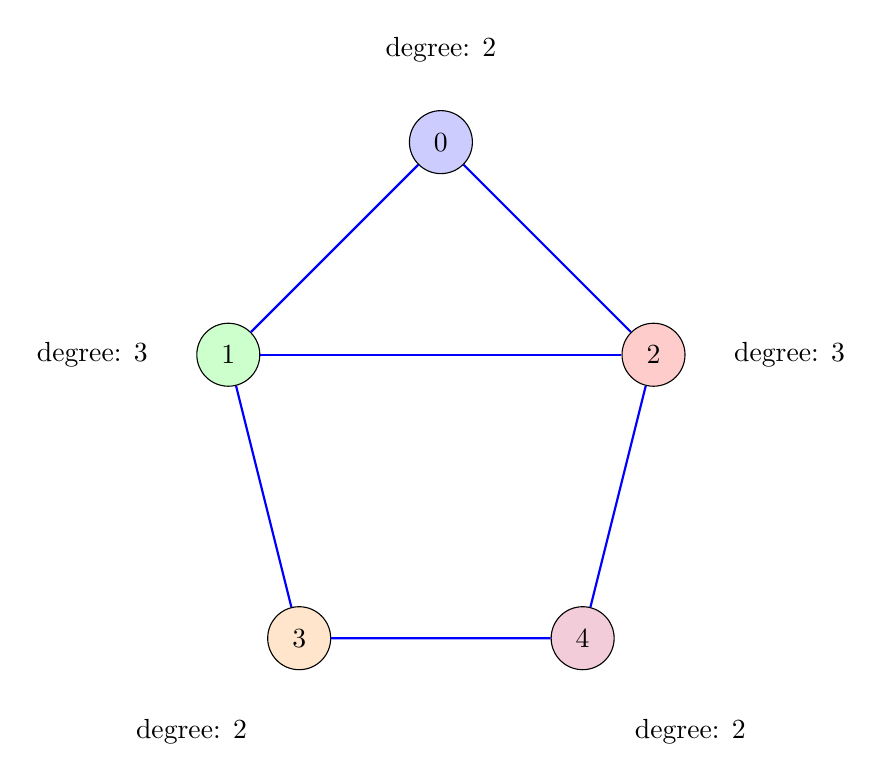
\begin{tikzpicture}[scale=1.8]
  % Define vertices
  \node[circle, draw, fill=blue!20, minimum size=0.8cm] (0) at (0,2) {0};
  \node[circle, draw, fill=green!20, minimum size=0.8cm] (1) at (-1.5,0.5) {1};
  \node[circle, draw, fill=red!20, minimum size=0.8cm] (2) at (1.5,0.5) {2};
  \node[circle, draw, fill=orange!20, minimum size=0.8cm] (3) at (-1,-1.5) {3};
  \node[circle, draw, fill=purple!20, minimum size=0.8cm] (4) at (1,-1.5) {4};

  % Draw edges
  \draw[thick, blue] (0) -- (1);
  \draw[thick, blue] (0) -- (2);
  \draw[thick, blue] (1) -- (2);
  \draw[thick, blue] (1) -- (3);
  \draw[thick, blue] (2) -- (4);
  \draw[thick, blue] (3) -- (4);

  % Add degree labels
  \node[above] at (0,2.5) {degree: 2};
  \node[left] at (-2,0.5) {degree: 3};
  \node[right] at (2,0.5) {degree: 3};
  \node[below left] at (-1.3,-2) {degree: 2};
  \node[below right] at (1.3,-2) {degree: 2};
\end{tikzpicture}
\end{document}
      